\documentclass[peerreview]{IEEEtran}
\usepackage{cite} % Tidies up citation numbers.
\usepackage{url} % Provides better formatting of URLs.
\usepackage[utf8]{inputenc} % Allows Turkish characters.
\usepackage{booktabs} % Allows the use of \toprule, \midrule and \bottomrule in tables for horizontal lines
\usepackage{graphicx}
\usepackage{xcolor}

\usepackage{listings}

\definecolor{mygreen}{rgb}{0,0.6,0}
\definecolor{mygray}{rgb}{0.5,0.5,0.5}
\definecolor{mymauve}{rgb}{0.58,0,0.82}

\lstdefinestyle{CStyle}{
  belowcaptionskip=1\baselineskip,
  breaklines=true,
  frame=L,
  xleftmargin=\parindent,
  language=C,
  showstringspaces=false,
  basicstyle=\footnotesize\ttfamily,
  keywordstyle=\bfseries\color{green!40!black},
  commentstyle=\itshape\color{purple!40!black},
  identifierstyle=\color{blue},
  stringstyle=\color{orange},
}

\hyphenation{op-tical net-works semi-conduc-tor} % Corrects some bad hyphenation 

\begin{document}
%\begin{titlepage}
% paper title
% can use linebreaks \\ within to get better formatting as desired
\title{System on Chip Architecture \\ Lab 1 Report}

% author names and affiliations

\author{Daniele Castro S253244\\
System-on-chip architecture\\
Politecnico of Turin\\
}
\date{26/12/2018}

% make the title area
\maketitle
\tableofcontents
\listoffigures
%\end{titlepage}

\IEEEpeerreviewmaketitle
\begin{abstract}
In this lab implemented a simple PSM (Power State Machine) using the MCU STM32F051R8 on the discovery board. The progect, as it is, is useles. It only gives me the possibility to develop simple functions to switch in various low power modes so that in more userfull projects I can reuse them. I also made some measurements for each low power mode so that I can estimate the lowest power consumption for each state with every peripheral switched off since I was not power on any of them.
\end{abstract}
\section{Introduction}
I am going to explain in sequence\\
1) The PSM states\\
2) How the transition happens\\
3) The code I wrote
\section{Background}
As described in the datasheet:\\
"The device features three low-power modes:
\begin{itemize}
\item Sleep mode (CPU clock off, all peripherals including Cortex®-M0 core peripherals like
NVIC, SysTick, etc. are kept running)
\item Stop mode (all clocks are stopped)
\item Standby mode (1.8V domain powered-off)"
\end{itemize}
As described in the Assignment:
\begin{itemize}
\item "SLEEP (WFI) mode is waken-up by any interrupt/event. In this case we use the user button to exit.
\item STOP mode requires RTC by setting EXTI line 17 that is connected to the RTC. We use RTC as we do not have EXTI source connected.
\item STANBY mode uses WKUP pin 1, that is PA.0 connected to the USER button. No RTC is used.
GPIO configuration is present in SLEEP and STOP, not present in STANDBY mode. \textcolor{red}{Because we have to reset after this state and we want to kind of stay off. We want power just to handle any reset event.} Wakeup source from Sleep and Stop mode is an EXTI Line configured in event mode. The wakeup source from
Standby mode is the WKUP1 pin (PA0)."
\end{itemize}
\section{Proposed Solution}
Since it is not possible to switch between low power states without passing in ACTIVE mode, I implemented the following PSM to switch between states.At power on the board waits for a user button pressure so that can it enter in the first low-power mode. then, once entered in STOP mode, waits for another user button pressure to exit from the current state. Once exited the board goes in sleep mode and exits from there after the RTC overflows. So we can, finally, go into standby mode. Here The user button pressure will cause a reset of the board. Note, also, the switching order:
\begin{figure}[!ht]
\centering
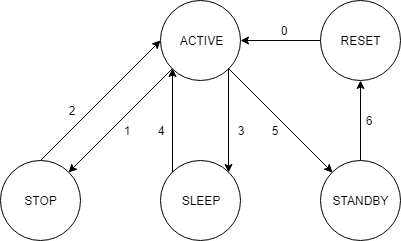
\includegraphics[width=0.8\columnwidth]{psm} 
\caption{Power State Machine}
\label{fig_sim}
\end{figure} 
\section{Results and discussion}
Here are shown some figures about measurement I did during the lab sessions that displayes current consumption of each low power state and active state
\begin{figure}[!ht]
\centering
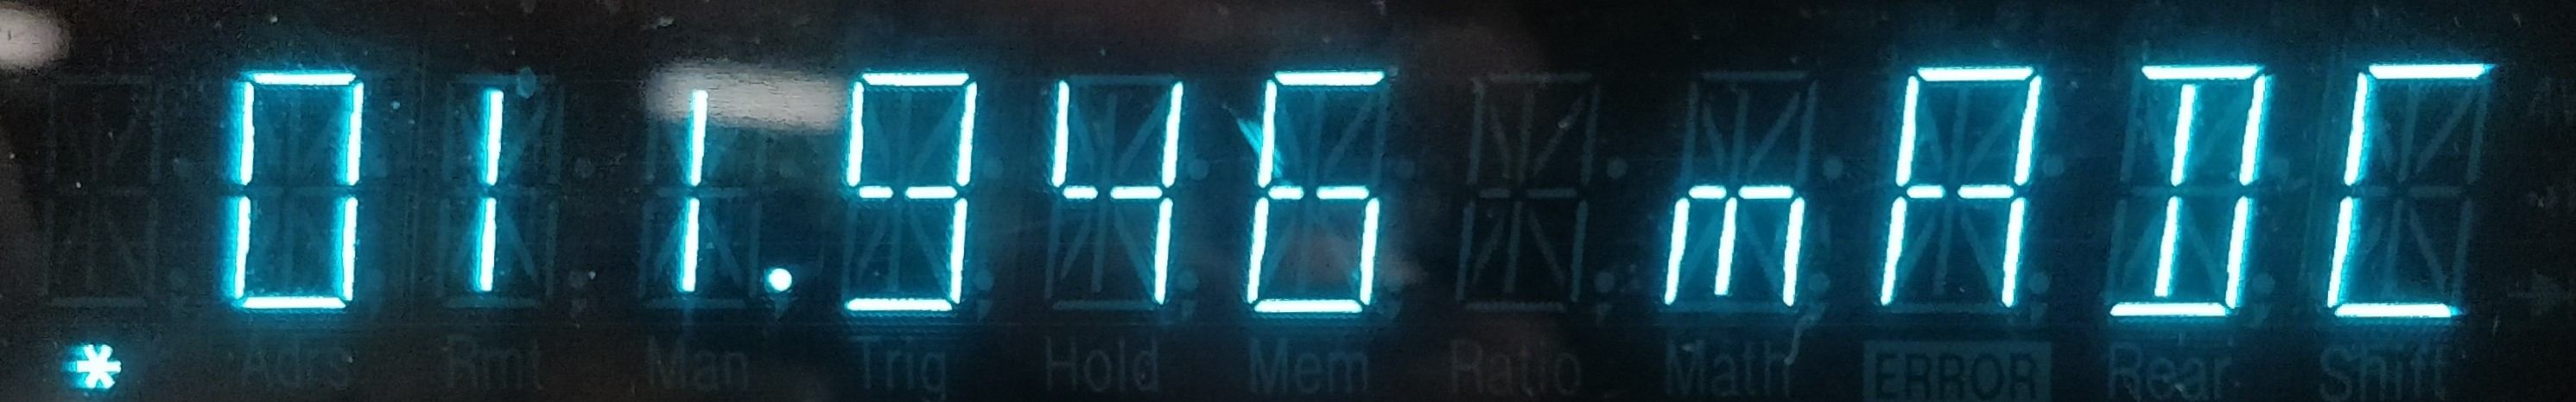
\includegraphics[width=0.7\columnwidth]{adc_active} 
\caption{Active mode power consumption}
\label{fig_A}
\end{figure}
\begin{figure}[!ht]
\centering
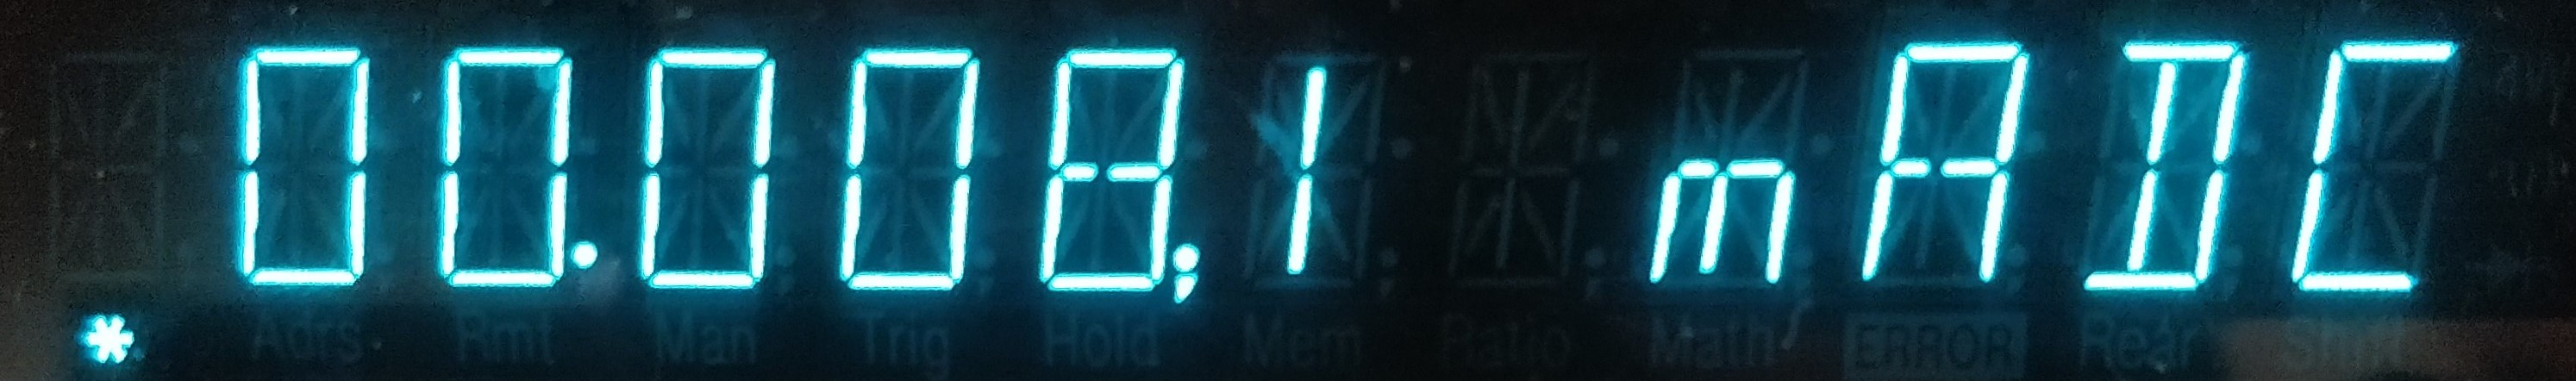
\includegraphics[width=0.7\columnwidth]{adc_stop} 
\caption{Stop mode power consumption}
\label{fig_B}
\end{figure}
\begin{figure}[!ht]
\centering
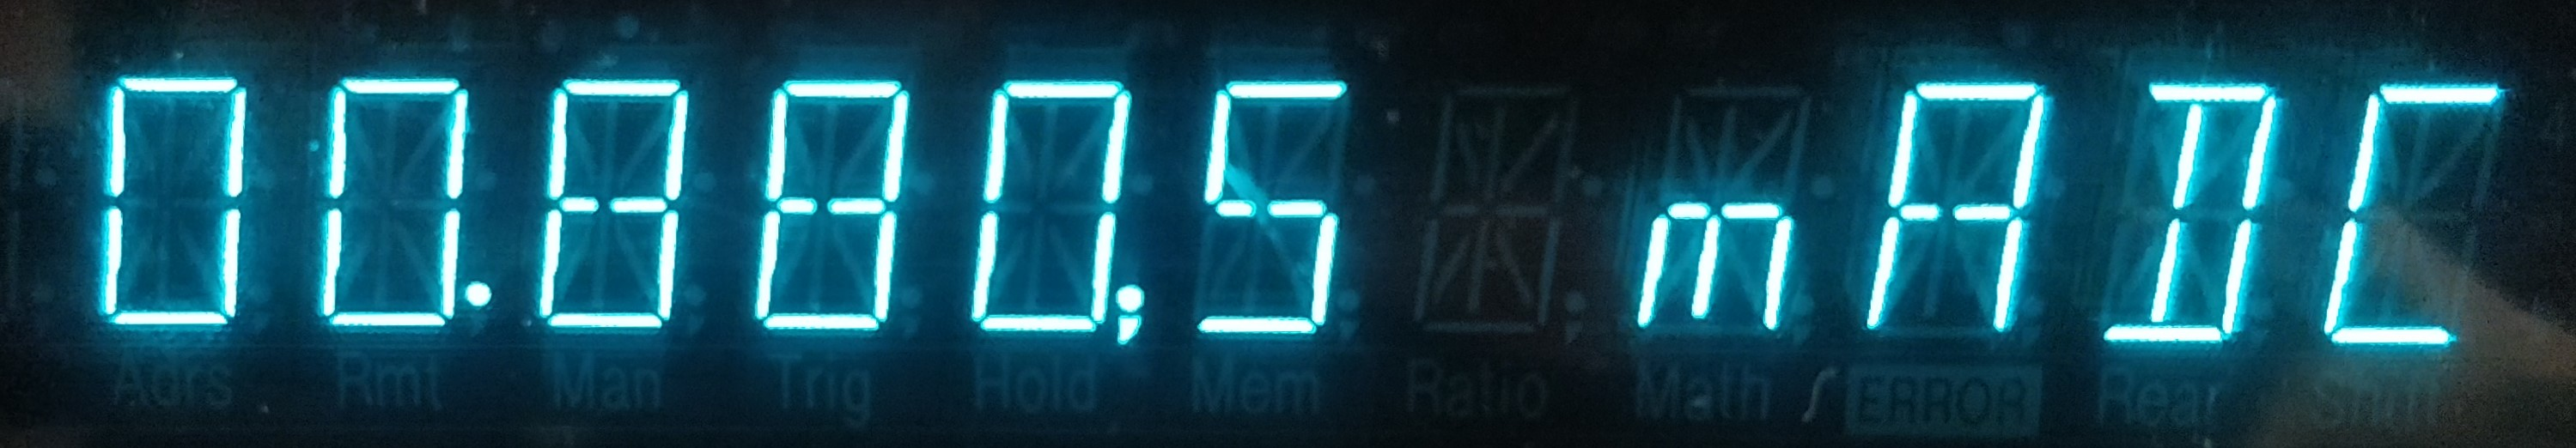
\includegraphics[width=0.7\columnwidth]{adc_sleep} 
\caption{Sleep mode power consumption}
\label{fig_C}
\end{figure}
\begin{figure}[!ht]
\centering
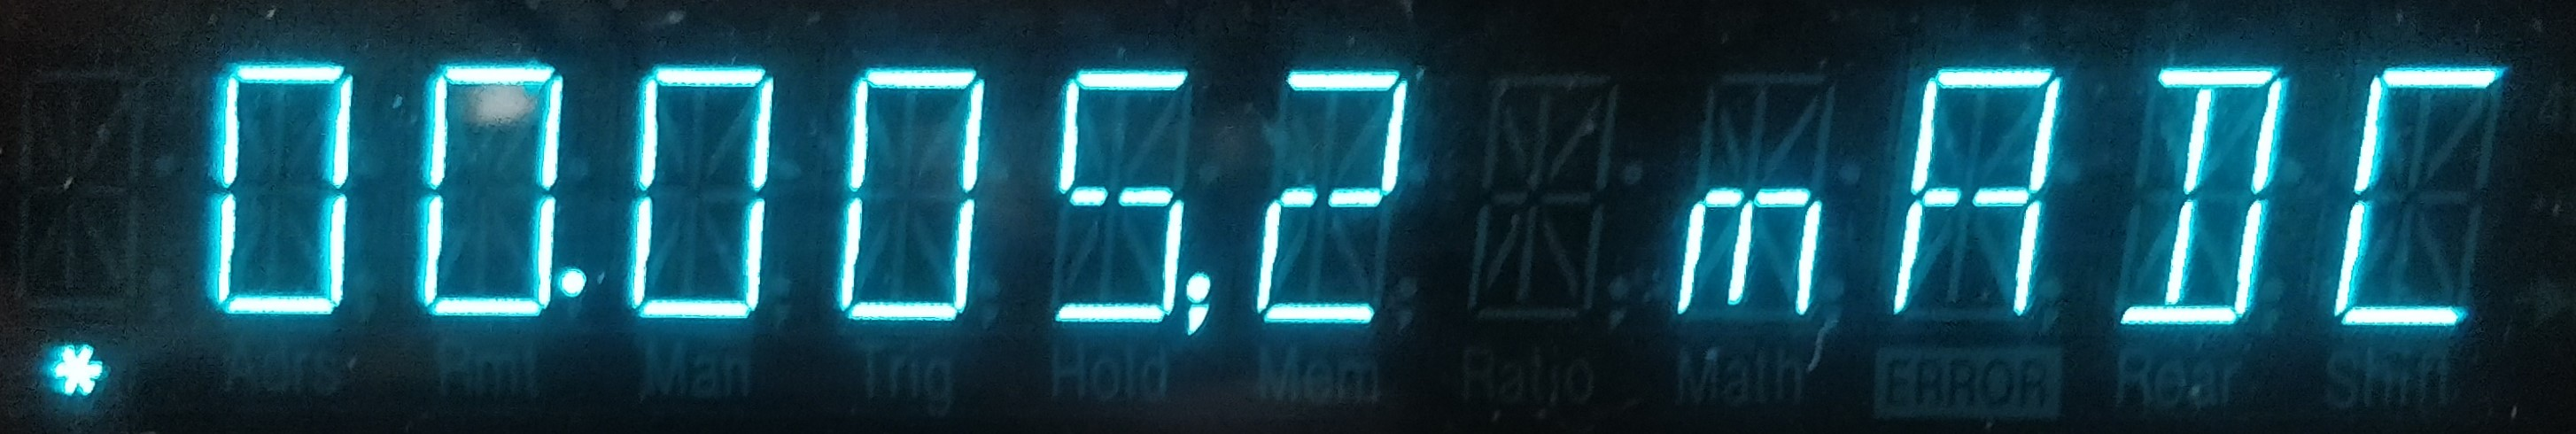
\includegraphics[width=0.7\columnwidth]{adc_standby} 
\caption{Standby mode power consumption}
\label{fig_D}
\end{figure}
\\Since I did not power on any peripheral, these results are good because they match values reported in the datasheet.\\
Looking at the code implementation I only commented out some \lstinline[style=CStyle]{while();} loops at the and of the functions 
\begin{lstlisting}[style=CStyle]
void SleepMode_Measure(void);
void StopMode_Measure(void);
\end{lstlisting}
so that, after wake up, I can move to active state and I can move to the next low power state. I also added:
\begin{lstlisting}[style=CStyle]
void led_modes(uint8_t mode, uint8_t times);
void UART2_init(void);
\end{lstlisting}
so that I can both flash green and blue LEDs on the board in four different patterns every time I switch between states and I can print on the serial terminal the specific name of the current state for debugging purposes. To do that I had to write down the low level implementations and declarations of
\begin{lstlisting}[style=CStyle]
#ifdef __GNUC__
  /* With GCC/RAISONANCE, small printf (option LD Linker->Libraries->Small printf
     set to 'Yes') calls __io_putchar() */
  #define PUTCHAR_PROTOTYPE int __io_putchar(int ch)
#else
  #define PUTCHAR_PROTOTYPE int fputc(int ch, FILE *f)
#endif /* __GNUC__ */
	
#ifdef __GNUC__
  /* With GCC/RAISONANCE, small printf (option LD Linker->Libraries->Small printf
     set to 'Yes') calls __io_putchar() */
  #define PUTCHAR_PROTOTYPE int __io_getchar(int ch)
#else
  #define GETCHAR_PROTOTYPE int fgetc(FILE *f)
#endif /* __GNUC__ */

...

PUTCHAR_PROTOTYPE
{
  /* fputc implementation: */
  /* write a character to the USART */
  USART_SendData(USART2, (uint8_t) ch);
  /* Loop until transmit data register is empty */
  while (USART_GetFlagStatus(USART2, USART_FLAG_TXE) == RESET)
  {}
  return ch;
}

GETCHAR_PROTOTYPE
{
	FILE *fd;
	char ch;
  /* fgetc implementation: */
  /* Loop until RXNE = 1 */
  while (USART_GetFlagStatus(USART2, USART_FLAG_RXNE) == RESET)
  {}
  /* read a character to the USART */
	ch = USART_ReceiveData(USART2);
	if(ch == '\r' || ch == '\n')	printf("\n\r");
	else fputc(ch, fd);
  return ch;
}
\end{lstlisting}
as result I obtained on the serial console a full listing of what is currently happening on the board:\\
\begin{figure}[!ht]
\centering
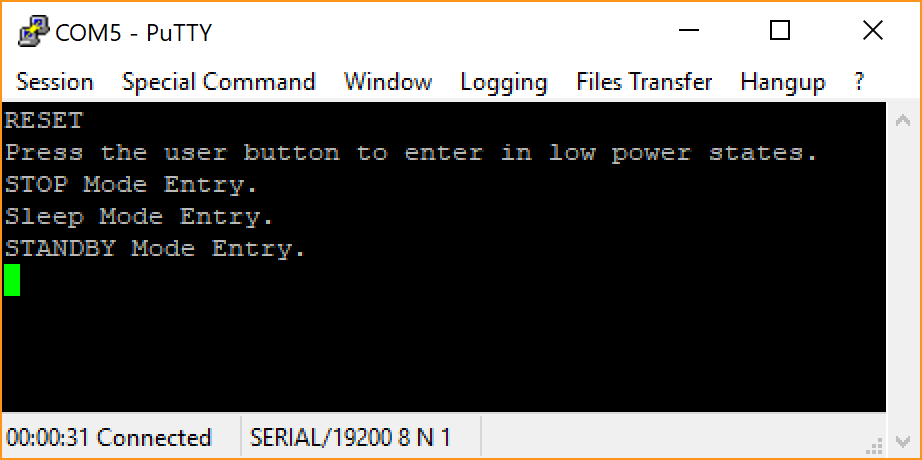
\includegraphics[width=0.8\columnwidth]{serial} 
\caption{Serial terminal window}
\label{fig_serial}
\end{figure}
\\Finally here is the piece of code I implemented to switch between all the states:
\begin{lstlisting}[style=CStyle]
printf("STOP Mode Entry.\n\r");
led_modes(3, 4);
...
StopMode_Measure();
	
UART2_init();
printf("Sleep Mode Entry.\n\r");
led_modes(2, 4);
...
SleepMode_Measure();
	
UART2_init();
printf("STANDBY Mode Entry.\n\r");
led_modes(0, 4);
...
StandbyMode_Measure(); //here it blocks and resets if user button pressed.

/*following code will never reached:*/
UART2_init();
printf("Exiting all of the modalities.\n\r");
led_modes(1, 4);
while(1);
\end{lstlisting}
\begin{lstlisting}[style=CStyle]
void StopMode_Measure(void);
\end{lstlisting}
\begin{itemize}
\item configures RTC
\item configures GPIO as analog to reduce current consumption
\item Disable GPIOs clock 
\item configures EXTI
\item configures NVIC
\item enables RTC
\item enters in STOP mode
\end{itemize}
Note that RTC (Real Time Clock) is clocked by a low power/frequency clock source called LSI that is an internal RC oscillator. It has also some registers called RCC That can control the clock source of this and other peripherals and save the current status when there is no power.
\begin{lstlisting}[style=CStyle]
void SleepMode_Measure(void);
\end{lstlisting}
\begin{itemize}
\item simply disables GPIO clock
\item configures user button in EXTI mode
\item enters in SLEEP mode
\end{itemize}
\begin{lstlisting}[style=CStyle]
void StandbyMode_Measure(void);
\end{lstlisting}
\begin{itemize}
\item sets PIN 2 as wake up PIN
\item enters in STANDBY mode
\end{itemize}
It's also important to notice that, has the name suggests, inside these functions
\begin{lstlisting}[style=CStyle]
void led_modes(uint8_t mode, uint8_t times);
void UART2_init(void);
\end{lstlisting}
I reinitialize each time the peripherals. Expecially the GPIO since it is all the times disabled by the low-power switching functions I mentioned above.\\
I also put an unreachable piece of code, as shown in the comments, that explains the fact that after exiting from the last power mode (standby) we can only reset.
\label{tab:template}

\section{Conclusions}
In this discussion I matched the assignment requests and, as an extra, I also properly configured the serial port to print debug messages and also eventually get strings from the input even if I didn't use it in this specific lab. I wish I will reuse these functions in future labs.
\end{document}